\section{Evaluation}

The problem set contains a mathematical test-bed and a set of practical application which should yield a good overview of the applicability of the different algorithms.


\subsection{Benchmarking functions}

The functions for the benchmark are taken from the 2005 CEC conference on continuous evolutionary optimization \cite{suganthan2005problem}. The functions are losely based on the popular optimization benchmark suite created by DeJong \cite{Whitley1996245}.

For all functions $x=[x_1,x_2,x_3,...,x_D]$ are the input parameters, $o=[o_1,o_2,o_3,...,o_D]$ is the global optimum, $D$ is the dimension and $M$ is an orthogonal matrix with parameters unique to each function. The matrices for $o$ and $M$ are available in appendix A. Illustrations of the functions can be found in figures \ref{f1}, \ref{f2}, \ref{f3}, \ref{f4}, \ref{f5}, \ref{f6}, \ref{f7}, \ref{f8}, \ref{f9} and \ref{f10}.

\subsubsection{$F_1$: Shifted Sphere Function}

\begin{equation}
  F_1(x)=\sum_{i=1}^{D}{z_i^2}
\end{equation}
\[ z=x-o \]
\[ x \in [-100,100]^D \]

\begin{figure}[H]
  \centering
  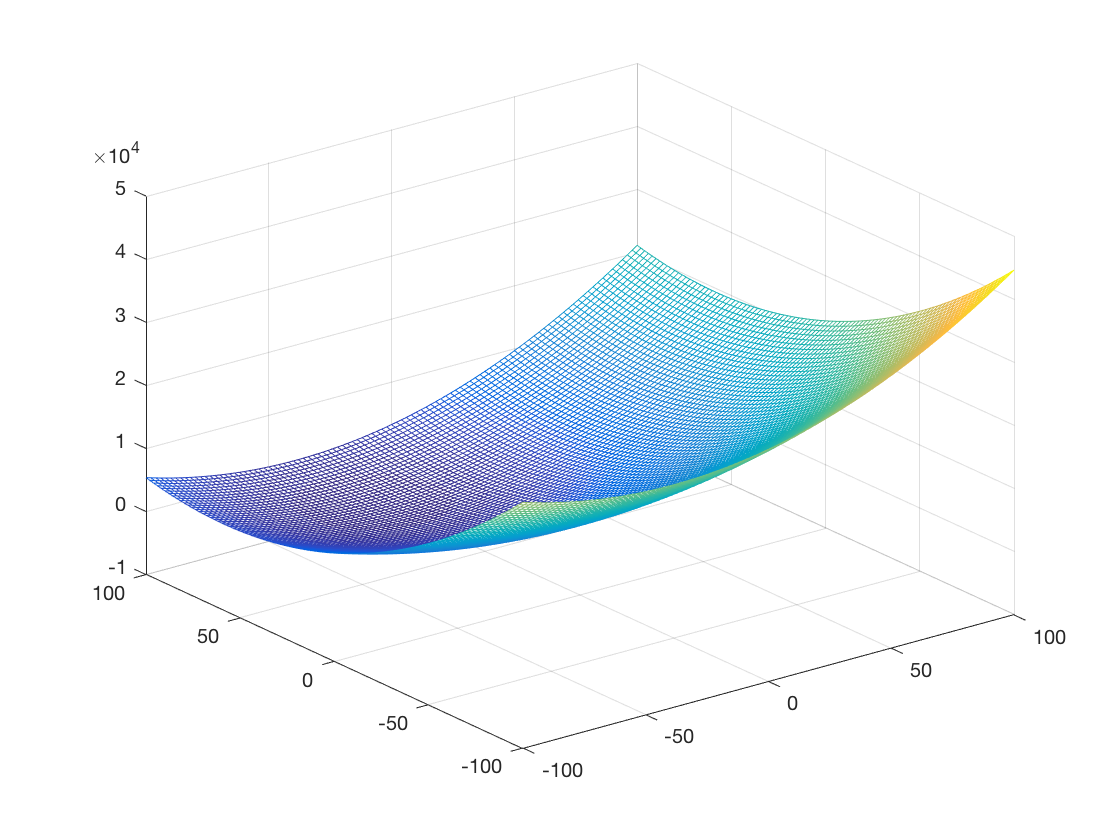
\includegraphics[width=.5\linewidth]{f1}
  \caption{3-D map for 2-D function}
  \label{f1}
\end{figure}

\subsubsection{$F_2$: Shifted Schwefel’s Problem}

\begin{equation}
  F_2(x)=\sum_{i=1}^{D}{(\sum_{j=1}^{i}{z_j})^2}
\end{equation}
\[ z=x-o \]
\[ x \in [-100,100]^D \]

\begin{figure}[H]
  \centering
  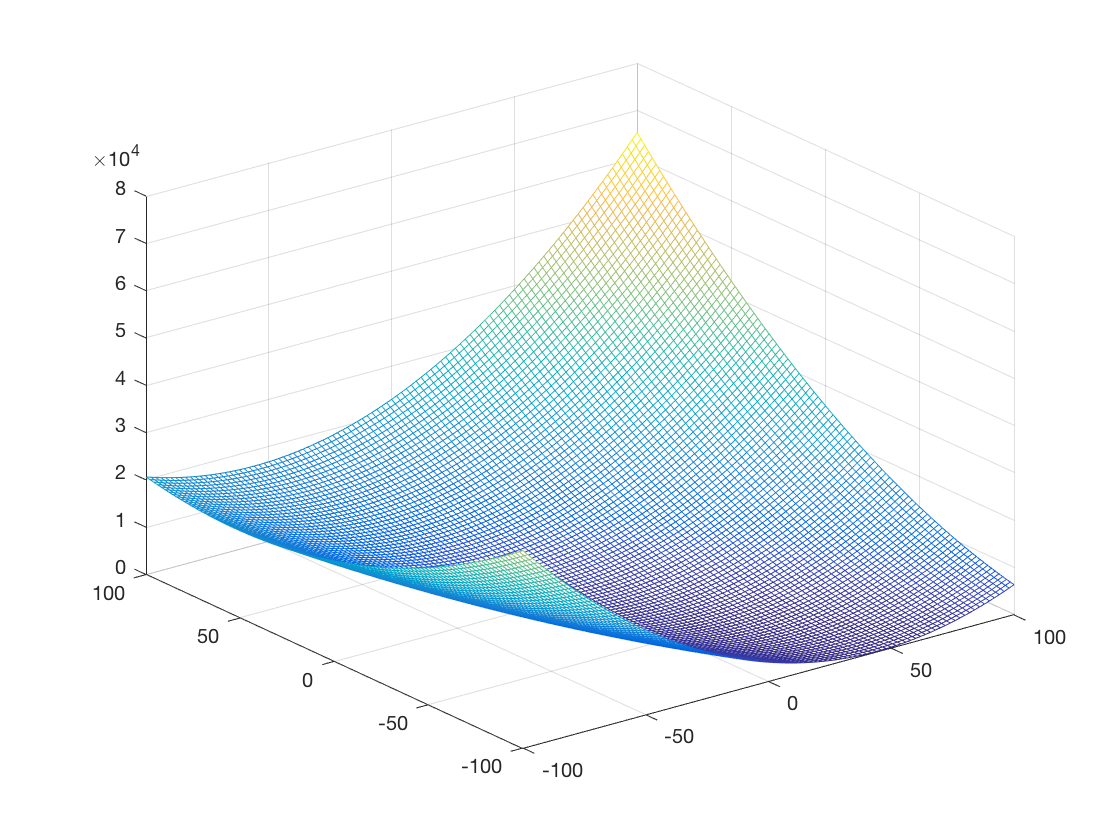
\includegraphics[width=.5\linewidth]{f2}
  \caption{3-D map for 2-D function}
  \label{f2}
\end{figure}

\subsubsection{$F_3$: Shifted Rotated High Conditioned Elliptic Function}

\begin{equation}
  F_3(x)=\sum_{i=1}^{D}{(10^6)^{\frac{i-1}{D-1}}z_i^2}
\end{equation}
\[ z=(x-o)*M \]
\[ x \in [-100,100]^D \]

\begin{figure}[H]
  \centering
  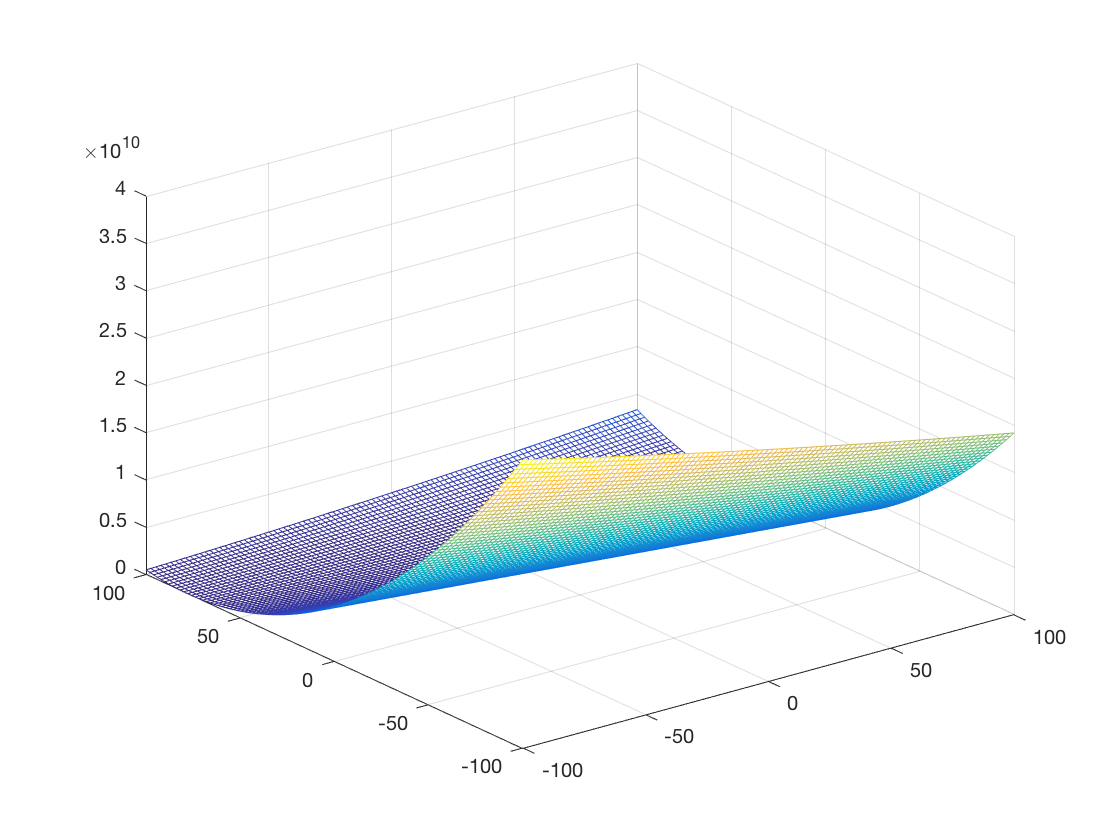
\includegraphics[width=.5\linewidth]{f3}
  \caption{3-D map for 2-D function}
  \label{f3}
\end{figure}

\subsubsection{$F_4$: Shifted Schwefel’s Problem with Noise in Fitness}

\begin{equation}
  F_4(x)=(\sum_{i=1}^{D}{(\sum_{j=1}^{i}{z_j})^2})*(1+0.4|N(0,1)|)
\end{equation}
\[ z=x-o \]
\[ x \in [-100,100]^D \]

\begin{figure}[H]
  \centering
  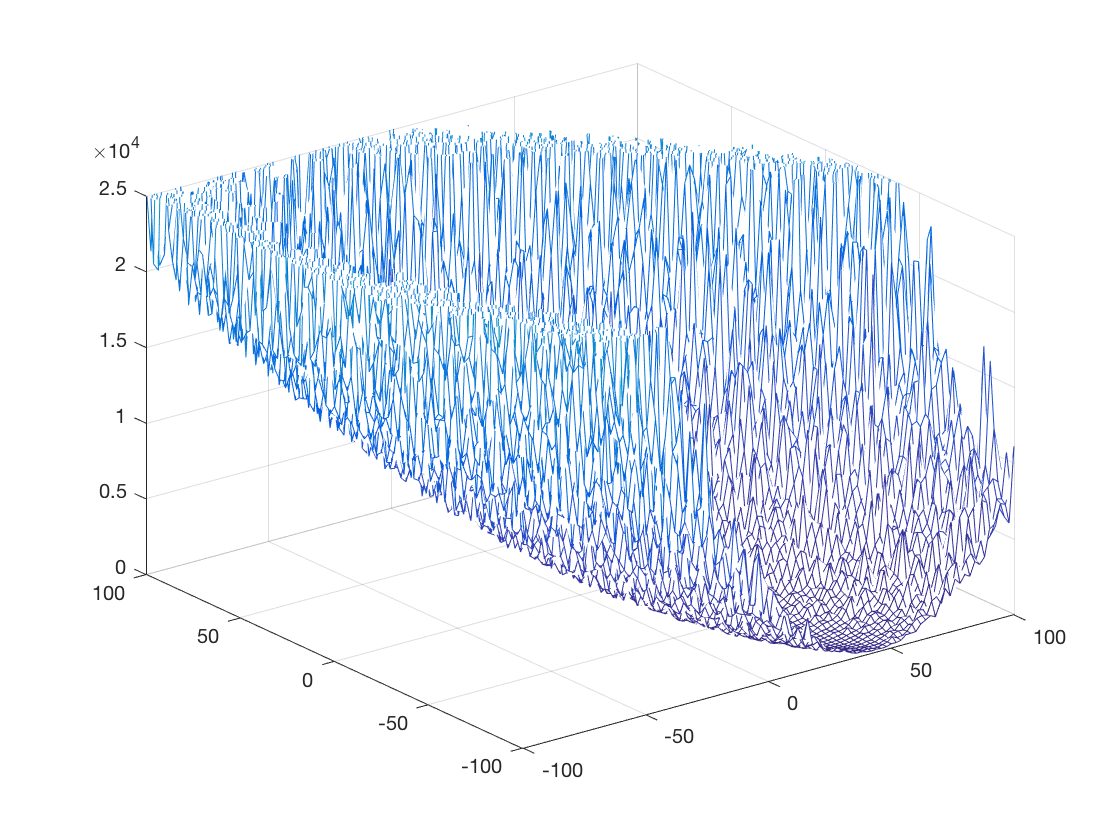
\includegraphics[width=.5\linewidth]{f4}
  \caption{3-D map for 2-D function}
  \label{f4}
\end{figure}

\subsubsection{$F_5$: Schwefel’s Problem with Global Optimum on Bounds}

\begin{equation}
  F_5(x)=max\{|A_ix-B_i|\}
\end{equation}
\[ i=1,...,D, x \in [-100,100]^D \]
\[ A \text{ is a } D*D \text{ matrix}, a_{ij} = \text{ random numbers in } [-500,500],  det(A) \neq 0 \]
\[ B_i = A_i * o, o_i = \text{ random numbers in } [-100,100] \]
\[ o_i = -100 \text{, for } i=1,2,...,[D/4], o_i = 100 \text{, for } i=[3D/4],...,D \]

\begin{figure}[H]
  \centering
  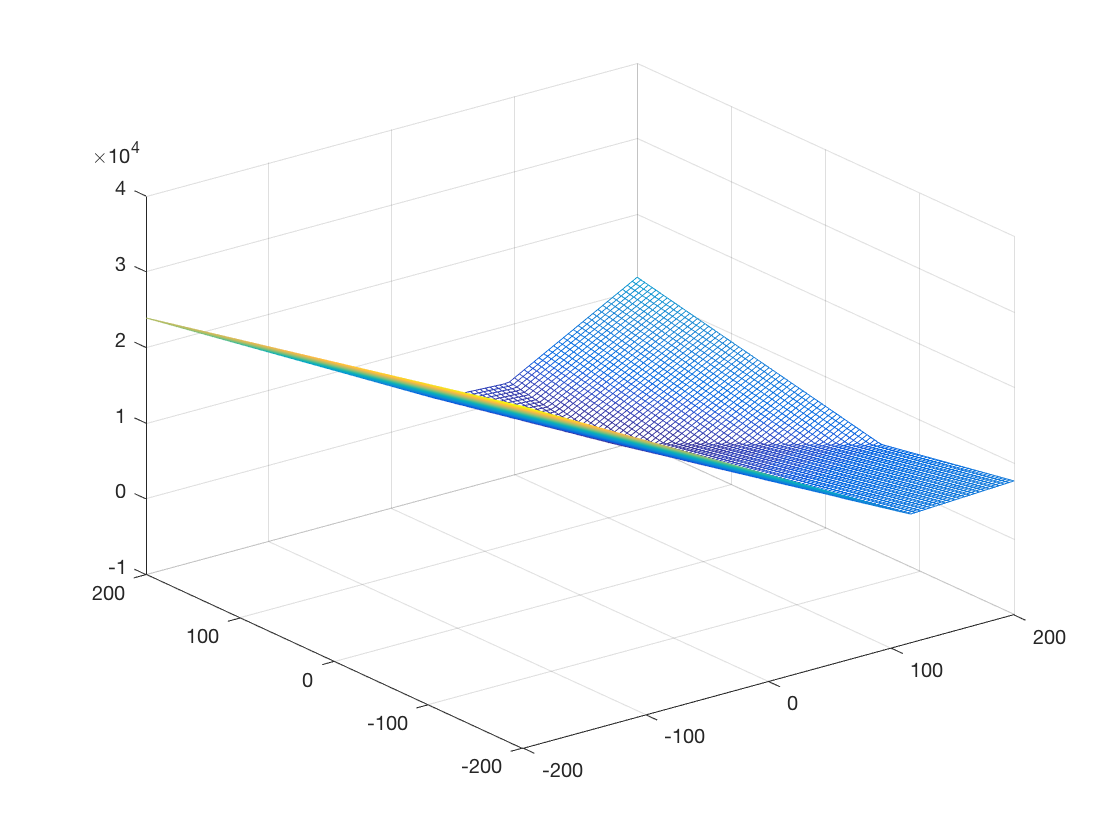
\includegraphics[width=.5\linewidth]{f5}
  \caption{3-D map for 2-D function}
  \label{f5}
\end{figure}

\subsubsection{$F_6$: Shifted Rosenbrock’s Function}

\begin{equation}
  F_6(x)=\sum_{i=1}^{D-1}{(100(z_i^2 - z_{i+1})^2 + (z_i - 1)^2)}
\end{equation}
\[ z=x-o+1 \]
\[ x \in [-100,100]^D \]

\begin{figure}[H]
  \centering
  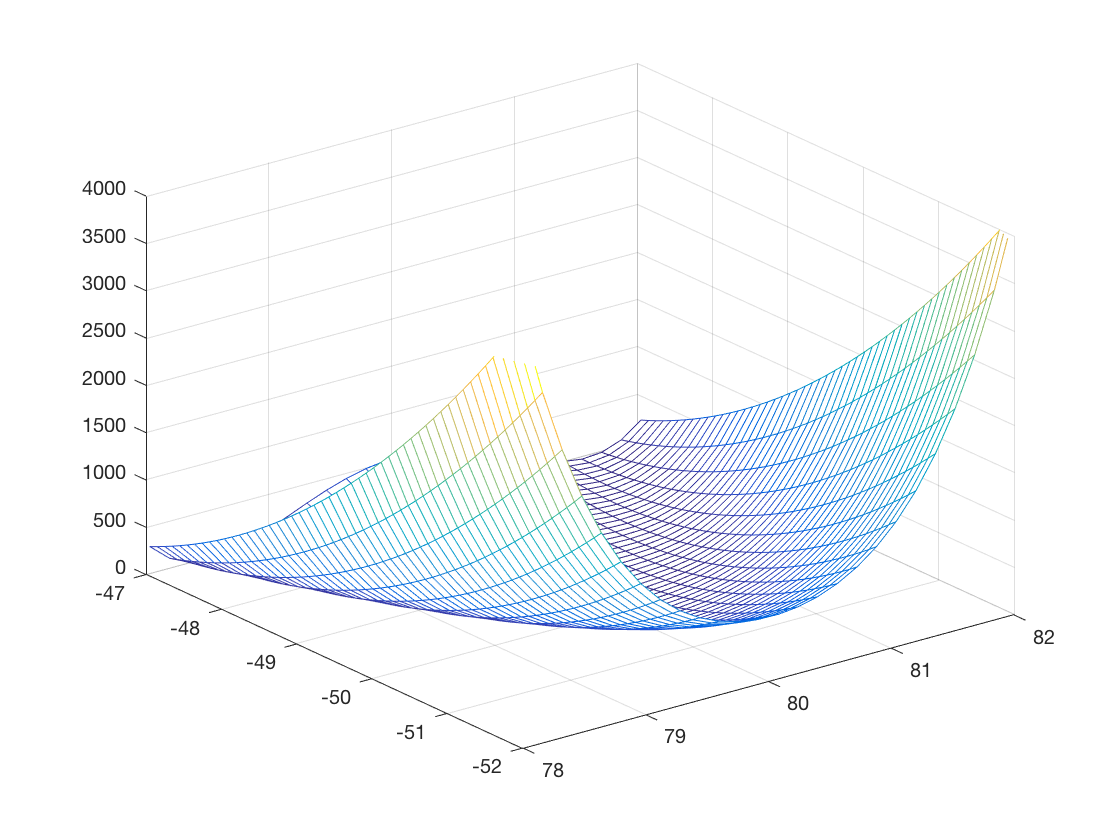
\includegraphics[width=.5\linewidth]{f6}
  \caption{3-D map for 2-D function}
  \label{f6}
\end{figure}

\subsubsection{$F_7$: Shifted Rotated Griewank’s Function without Bounds}

\begin{equation}
  F_7(x)=\sum_{i=1}^{D}{\frac{z_i^2}{4000}}-\prod_{i=1}^{D}{\cos{\frac{z_i}{\sqrt{i}}}}+1
\end{equation}
\[ z=(x-o)*M \]
\[ x \in [0,600]^D \]

\begin{figure}[H]
  \centering
  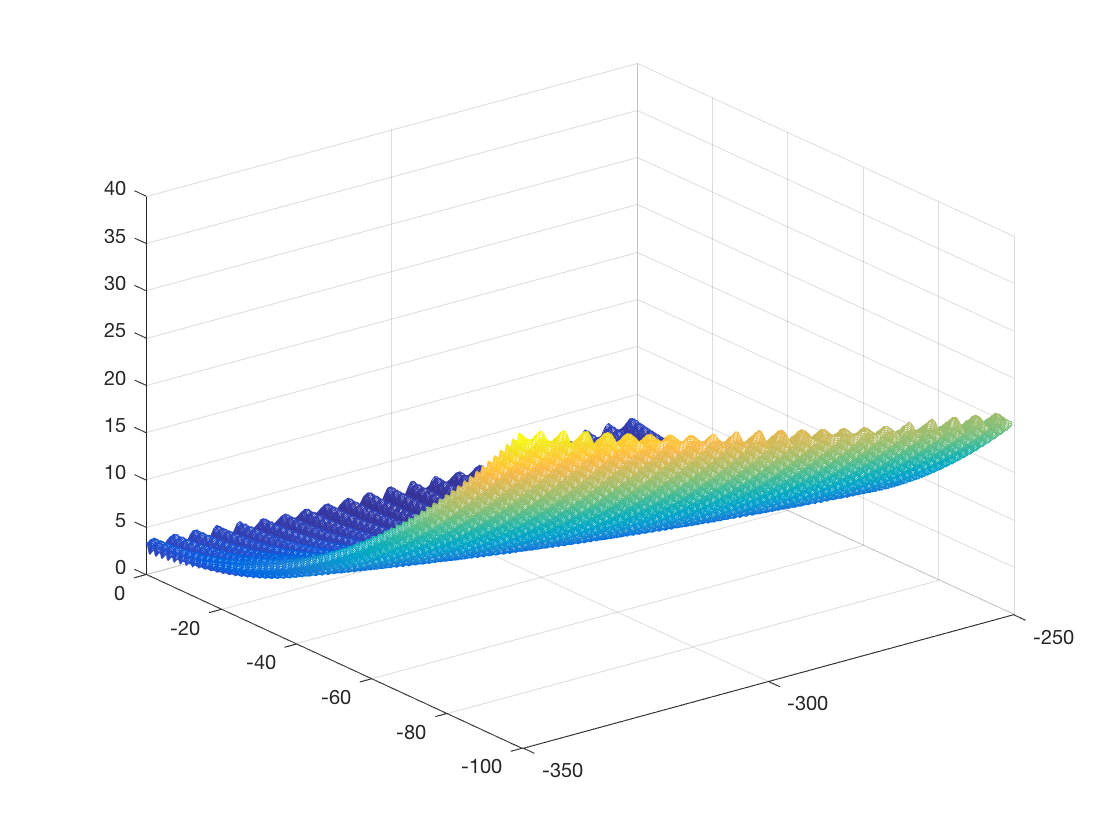
\includegraphics[width=.5\linewidth]{f7}
  \caption{3-D map for 2-D function}
  \label{f7}
\end{figure}

\subsubsection{$F_8$: Shifted Rotated Ackley’s Function with Global Optimum on Bounds}

\begin{equation}
  F_8(x)=-20\exp{(-0.2\sqrt{\frac{1}{D}\sum_{i=1}^{D}{z_i^2}})}-\exp{(\frac{1}{D}\sum_{i=1}^{D}{\cos{(2\pi z_i)}})} + 20 + e
\end{equation}
\[ z=(x-o)*M \]
\[ x \in [-32,32]^D \]

\begin{figure}[H]
  \centering
  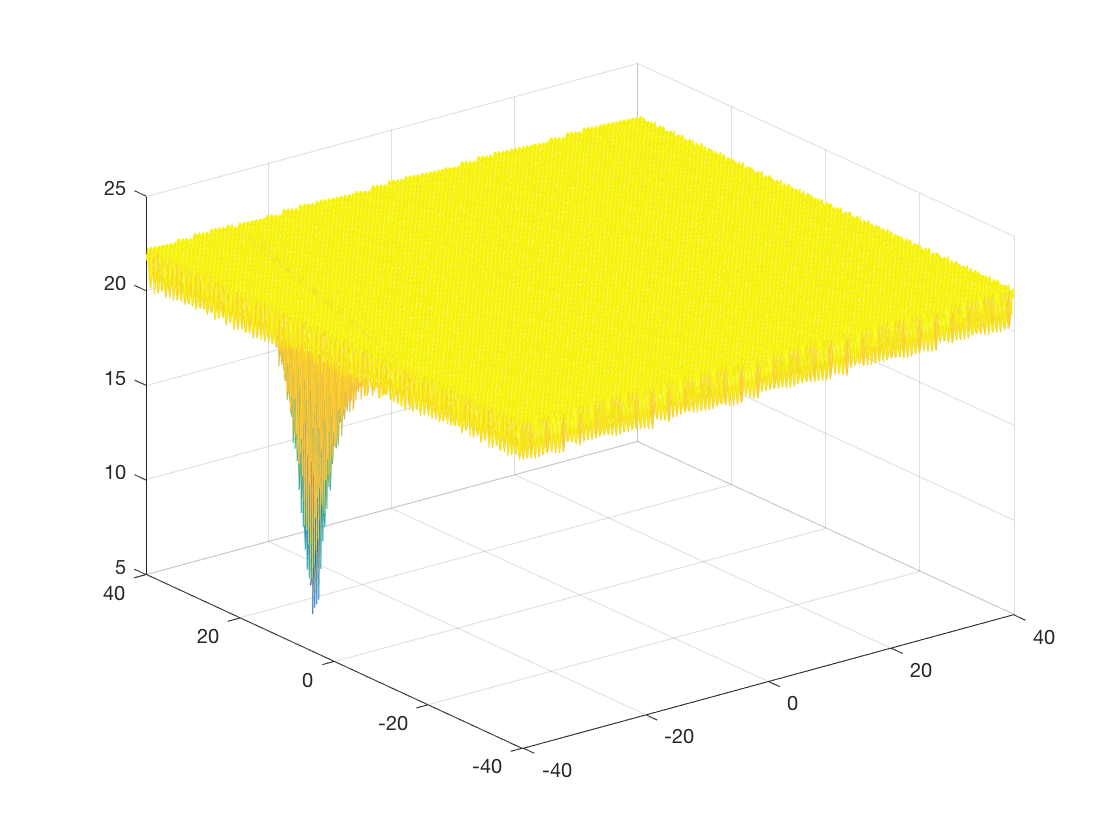
\includegraphics[width=.5\linewidth]{f8}
  \caption{3-D map for 2-D function}
  \label{f8}
\end{figure}

\subsubsection{$F_9$: Shifted Rastrigin’s Function}

\begin{equation}
  F_9(x)=\sum_{i=1}^{D}{z_i^2 - 10\cos{(2\pi z_i)} + 10}
\end{equation}
\[ z=x-o \]
\[ x \in [-5,5]^D \]

\begin{figure}[H]
  \centering
  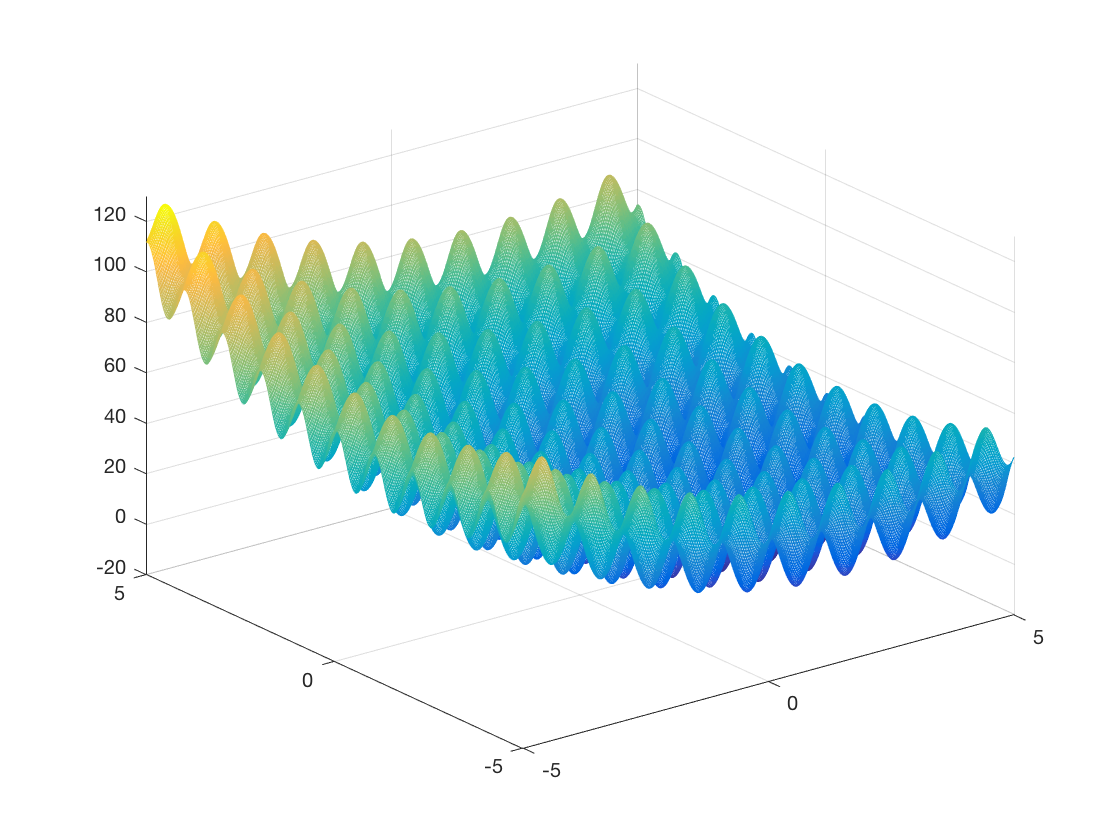
\includegraphics[width=.5\linewidth]{f9}
  \caption{3-D map for 2-D function}
  \label{f9}
\end{figure}

\subsubsection{$F_{10}$: Shifted Rotated Rastrigin’s Function}

\begin{equation}
  F_{10}(x)=\sum_{i=1}^{D}{z_i^2 - 10\cos{(2\pi z_i)} + 10}
\end{equation}
\[ z=(x-o)*M \]
\[ x \in [-5,5]^D \]

\begin{figure}[H]
  \centering
  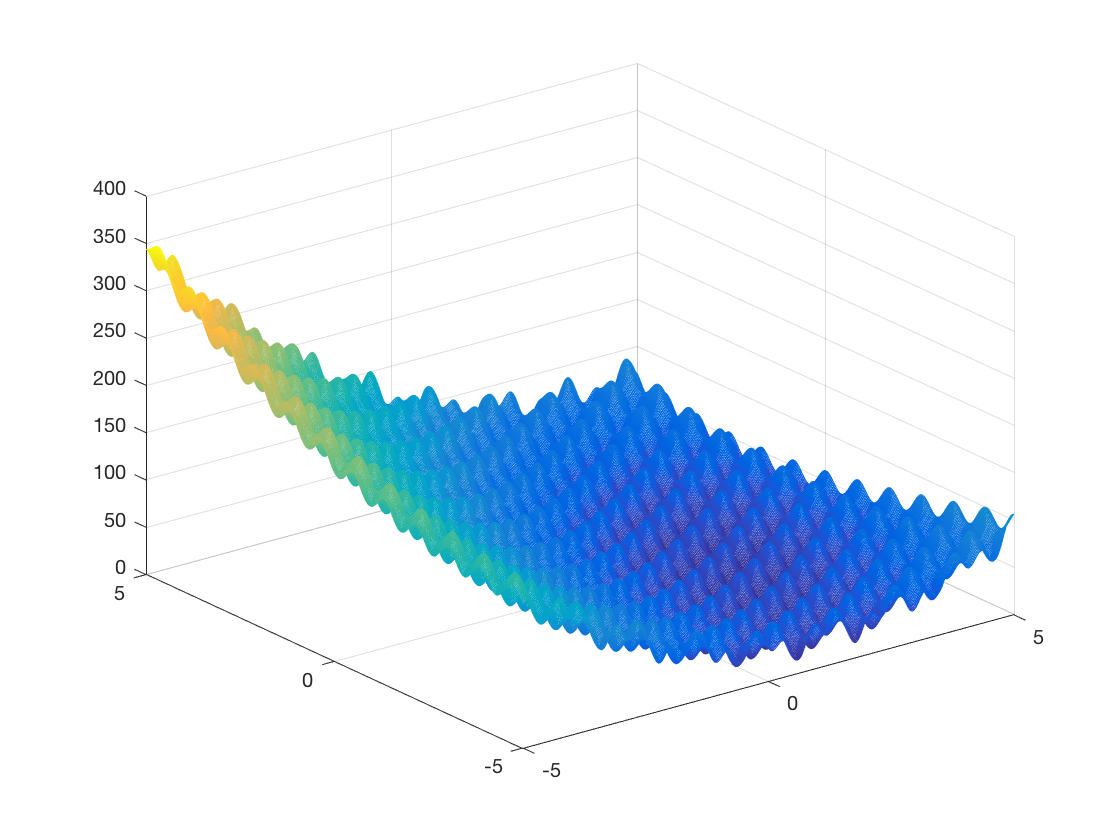
\includegraphics[width=.5\linewidth]{f10}
  \caption{3-D map for 2-D function}
  \label{f10}
\end{figure}

\subsection{Training neural networks}

Artificial neural networks usually consist of the following components:

\begin{enumerate}
  \item A graf of nodes (neurons) and links between nodes
  \item A variable for each neuron which contains it's value
  \item A real weight for each link between nodes
  \item A real threshold for each node
  \item A transfer function which calculates the value of each neuron based on other neurons variables, link-weights and thresholds
\end{enumerate}

Feed-Forward neural networks contain one level of input-nodes, one or more levels of hidden nodes and one level of output-nodes. The input-nodes accept an incomming singla vector and the output-neurons transmit the output-vector back to the user. All node in each level are linked to all other nodes in the previous and next levels \cite{montana1989training}. See figure \ref{figure:FFNN} for an illustration of a simple FFNN with two input nodes ($z_1$ and $z_2$), three hidden nodes ($y_1$, $y_2$ och $y_3$), two ouput nodes ($o_1$ och $o_2$) and weights between them represented by $v_{ij}$ and $w_{ij}$.

\subsubsection{Evaluating the network}

The value of neuron $x_i$ in the network is calculated according to the following equations

\begin{equation}
  x_i = f(\xi_i)
  \label{neuron}
\end{equation}

\begin{equation}
  \xi_i = v_i + \sum_{j = 0}^{n} {\omega_{ij}x_{j}}
  \label{neuron_sum}
\end{equation}

\noindent
where $n$ is the number of neurons in the previous layer, $x_j$ are neurons in the previous layer and $v_i$ are the weights between $x_i$ and $x_j$.

The function $f$ is the transfer-function and is defined according to

\begin{equation}
  f(\xi) = \frac {1} {1 + exp(-\xi)}
\end{equation}

To simplify the notation the threshold is added to the network as an additional node to all layers except the output-layer with a constant value of $-1$. The threshold values are the determined by the outgoing weights from the threshold nodes \cite{svozil1997introduction}.



\begin{figure}[H]
  \centering
    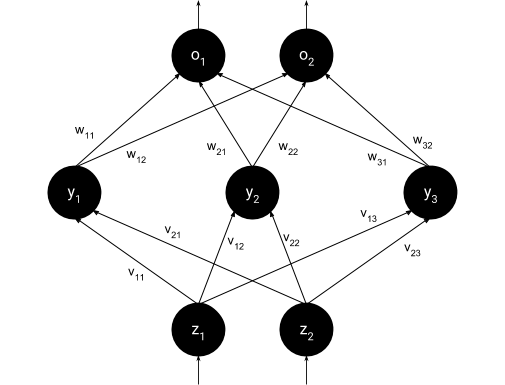
\includegraphics[width=10cm]{FFNN}
  \caption{Feed-Forward Neural Network}
  \label{figure:FFNN}
\end{figure}


\subsubsection{Backpropagation}

Backpropagation is the most popular method to train neural networks. Training-data is sent through the network and the result-vector is subtracted from the correct output-vector, squared and summed. The sum of squared differences is the propagated back through the network assigning a delta value to each node. Then new weights are calculated for each link based on the nodes delta values and the derivative of the transfer function. After a large enough number iterations the network will have learnt to correctly process the traning data and make correct predictions for all data in general \cite{engelbrecht2007computational}.
